
%%%%%%%%%%%%%%%%%%%%%%%%%%%%%%%%%%%%%%%%%%%%%%%%%%%%%%%%%%%%%%%%%%%%%%%%%
%           Capítulo 3: Control               %
%%%%%%%%%%%%%%%%%%%%%%%%%%%%%%%%%%%%%%%%%%%%%%%%%%%%%%%%%%%%%%%%%%%%%%%%%

\chapter{\textcolor{Azul}{Control}}
En este capítulo, se presenta la introducción al desarrollo de la tesis, ya sea el modelo matemático o las bases del proyecto, etc.
%Ejemplo de cita  [\citet{latex}]
%Ejemplo de cita [\citeauthor{RR73}]
 % The \cite command functions as follows:
 %   \citet{key} ==>>                Jones et al. (1990)
 %   \citet*{key} ==>>               Jones, Baker, and Smith (1990)
 %   \citep{key} ==>>                (Jones et al., 1990)
 %   \citep*{key} ==>>               (Jones, Baker, and Smith, 1990)
 %   \citep[chap. 2]{key} ==>>       (Jones et al., 1990, chap. 2)
 %   \citep[e.g.][]{key} ==>>        (e.g. Jones et al., 1990)
 %   \citep[e.g.][p. 32]{key} ==>>   (e.g. Jones et al., p. 32)
 %   \citeauthor{key} ==>>           Jones et al.
 %   \citeauthor*{key} ==>>          Jones, Baker, and Smith
 %   \citeyear{key} ==>>             1990

%%%%%%%%%%%%%%%%%%%%%%%%%%%%%%%%%%%%%%%%%%%%%%%%%%%%%%%%%%%%%%%%%%%%%%%%%
%                          Descripción de la planta                     %
%%%%%%%%%%%%%%%%%%%%%%%%%%%%%%%%%%%%%%%%%%%%%%%%%%%%%%%%%%%%%%%%%%%%%%%%%
\section{Conceptos de control}

A pesar de la existencia de robots comerciales de tipo industrial, diseñar controladores para robots sigue siendo un área compleja y constantemente estudiada por parte de los constructores de robots, así como por centros de investigación en control y robótica alrededor del mundo. Podría argumentarse que los robots industriales actuales son capaces de realizar correctamente una gran variedad de tareas, por lo que pareciera innecesario el desarrollo de investigaciones sobre el tema de control de robots. Sin embargo, este último tema, además de interesante, tiene muchos retos que ofrecer en el marco teórico, y más importante aún, su estudio es indispensable en aplicaciones específicas que no pueden ser llevadas a cabo mediante los robots comerciales actuales.\\

La metodología de diseño de los sistemas de control puede resumirse en los siguientes pasos:

\begin{itemize}
	\item Familiarización con el sistema físico a controlarse.
	\item Modelado.
	\item Especificaciones de control.
\end{itemize}

\subsection{Familiarización con el sistema fisico a controlarse}

En esta primera etapa deben identificarse las \textit{salidas del sistema}, que son todas aquellas variables físicas que se desea gobernar, tales como velocidad, desplazamiento, temperatura, etc. Además deben identificarse claramente aquellas variables físicas del sistema que se encuentran disponibles y que influyen en el comportamiento del mismo, y en particular afectan a las salidas del sistema. Estas variables llamadas \textit{entradas del sistema} pueden ser, por ejemplo, corriente eléctrica, par o fuerza, tensión, etc.\\

En el caso de los robots manipuladores, la variable de salida (denotada momentaneamente por $\textbf{y}$) cuya conducta se desea modificar, ofrece un amplio espectro de elecciones tal como podemos ver a continuación.\\

En el caso de robots que se desplazan libremente por un espacio de trabajo, tales como los destinados a tareas de pintado, traslado de objetos de un punto a otro, corte por rayo láser, etc, la salida del sistema $\textbf{y}$ puede corresponder simplemente a las velocidades $\textbf{q}$ y velocidades $\dot{\textbf{q}}$ articulares, o tambien la posición y orientación del efector final o herramienta.\\

\begin{figure}[h!]
	\centering
	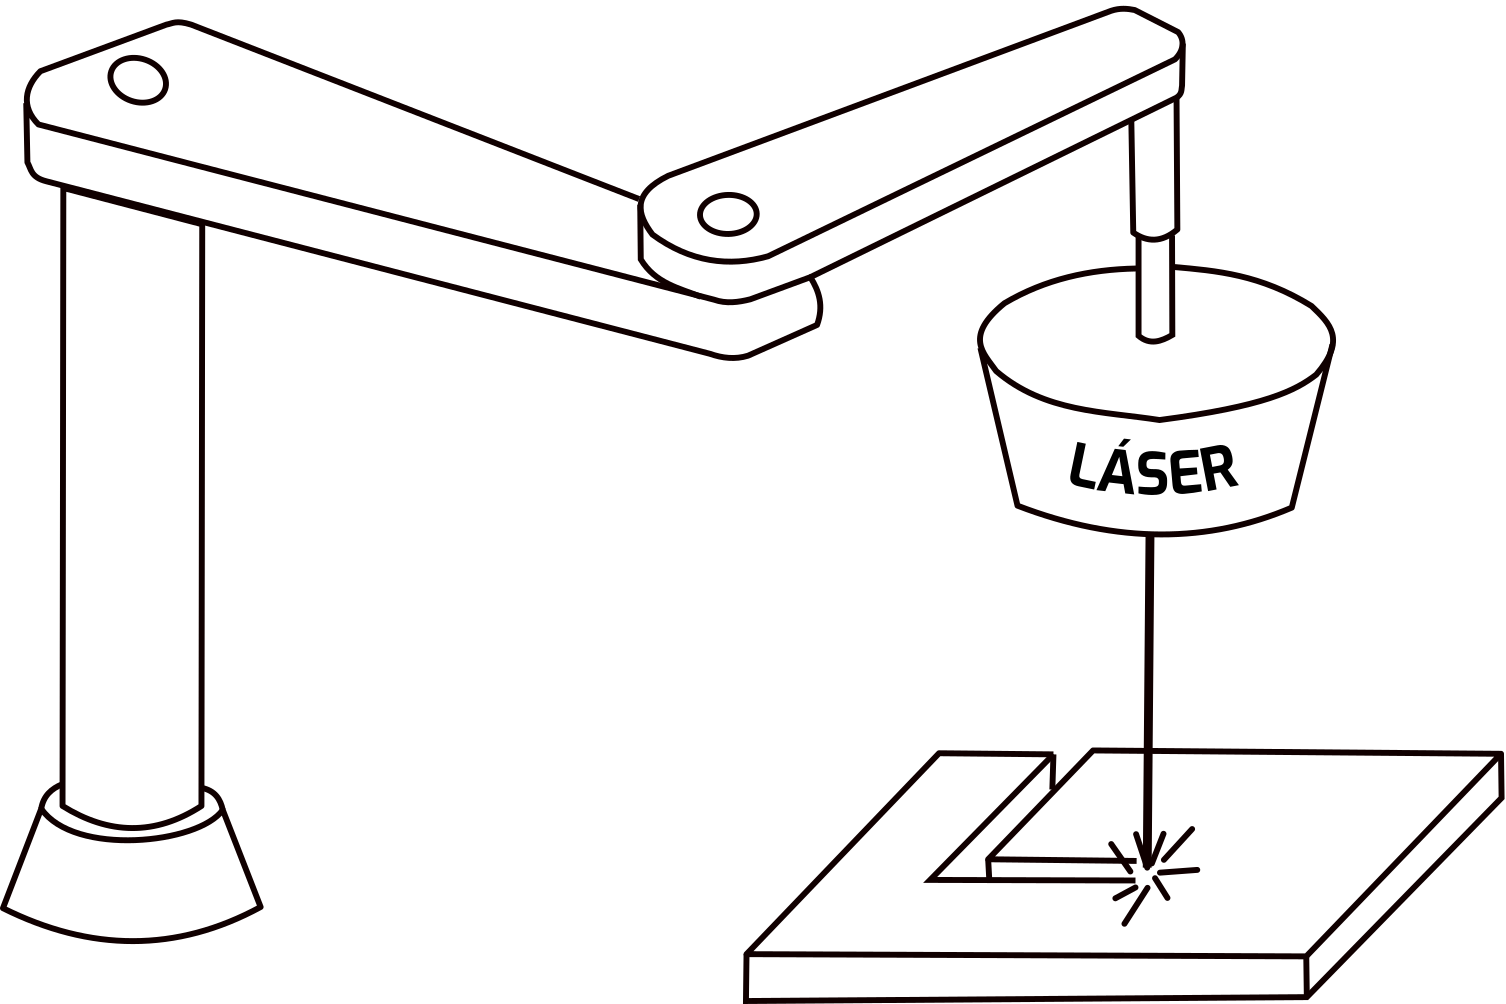
\includegraphics[scale=0.4]{Capitulo3/figs/robotLaser.png} 
	\caption{Robot en movimiento libre}
	\label{laser}
\end{figure}

\subsection{Modelado dinámico}


\subsection{Especificaciones de control}

%Ejemplo de cita \citep{texbook}


%%%%%%%%%%%%%%%%%%%%%%%%%%%%%%%%%%%%%%%%%%%%%%%%%%%%%%%%%%%%%%%%%%%%%%%%%
%                          Modelado                                     %
%%%%%%%%%%%%%%%%%%%%%%%%%%%%%%%%%%%%%%%%%%%%%%%%%%%%%%%%%%%%%%%%%%%%%%%%%
\section{Esquemas de control}

\subsection{PID}

\section{Control por par calculado}

\section{Parámetros de diseño}
Antes de comenzar, se definen  en la tabla ~\ref{tab:tabla} los parámetros y variables utilizadas

%%%%%%%%Tabla Nombres de parámetros
\begin{table}[htdp]                             %Inicia el entorno table debajo del texto
\centering\                                     %   centra la tabla
\begin{tabular}{||c | c ||}                     %inicia entorno tabular con doble línea en las orillas, 2 columnas con el contenido centrado (c)
\hline                                          %inserta línea horizontal
\hline
Nombre Parámetro/Variable & Símbolo\\
\hline
\hline
Masa del péndulo & $m$ \\
\hline
Masa del carro & $M$\\
\hline
Distancia del eje de giro al centro de masa & $l$ \\
\hline
Aceleración gravitatoria & $g$ \\
\hline
Momento de inercia péndulo respecto del eje de giro& $J$ \\
\hline
Ángulo del péndulo respecto del eje vertical & $\theta$\\
\hline
Velocidad angular del péndulo & $\dot{\theta}$, $\omega$\\
\hline
Distancia del carro respecto al centro del riel & x\\
\hline
Velocidad del carro & $\dot{x}$, $v$\\
\hline
\hline
\end{tabular}
\caption[Tabla 1]{\textbf{Parámetros dinámicos del carro-péndulo} - Estos son los valores de parámetros utilizados en el diseño y las simulaciones, corresponden a los valores reales.}
\label{tab:tabla}                              %etiqueta para referencia
\end{table}
